\chapter{A Non-Equilibrium Green's Function (NEGF) Based Magnetic Tunnel Junction (MTJ) Simulator in MATLAB\texttrademark}

\section{Introduction}

The Non-Equilibrium Green's Function (NEGF) based transport model was proposed in \cite{Salahuddin2007e,Datta2012b}. This document presents an implementation of a MATLAB\texttrademark{} based solver that calculates the $I-V$ characteristics of a magnetic tunnel junction (MTJ) using the proposed model. The NEGF model is based on the single band effective mass Hamiltonian ($\mathcal{H}$) and self-energy ($\Sigma_{L,R}$) which are used to calculate Green's function ($G$), electron correlation matrix ($G^n$) and charge current density ($J$). Fig.~\ref{fig:negf_grid} shows the device structure and coordinate system used for modeling MTJs. In a 1-D system, the Hamiltonian may be written for five regions: (a) the left ferromagnet (FM) contact, (b) the right FM contact, (c) the oxide channel, (d) the left FM-oxide interface, and (d) the right oxide-FM interface. Generally, the Hamiltonian, $\mathcal{H}$, may be written as \begin{equation}
\mathcal{H}=\left[\begin{IEEEeqnarraybox}[\scriptsize][c]{/c/c/c/c/c/c/c/c/c/c/c/}
\alpha_{HL1} & \beta_{HL1} & 0 & \cdots & \cdots & \cdots & \cdots & \cdots & \cdots & \cdots & 0 \\
\beta^{\dagger}_{HL1} & \ddots & \ddots & \ddots & ~ & ~ & ~ & ~ & ~ & ~ & \vdots \\
0 & \ddots & \alpha_{HL1} & \beta_{HL1} & \ddots & ~ & ~ & ~ & ~ & ~ & \vdots \\
\vdots & \ddots & \beta^{\dagger}_{HL1} & \alpha_{IL} & \beta_{OX} & \ddots & ~ & ~ & ~ & ~ & \vdots \\
\vdots & ~ & \ddots & \beta^{\dagger}_{OX} & \alpha_{OX} & \ddots & \ddots & ~ & ~ & ~ & \vdots \\
\vdots & ~ & ~ & \ddots & \ddots & \ddots & \ddots & \ddots & ~ & ~ & \vdots \\
\vdots & ~ & ~ & ~ & \ddots & \ddots & \alpha_{OX} & \beta_{OX} & \ddots & ~ & \vdots \\
\vdots & ~ & ~ & ~ & ~ & \ddots & \beta^{\dagger}_{OX} & \alpha_{IR} & \beta_{HL2} & \ddots & \vdots \\
\vdots & ~ & ~ & ~ & ~ & ~ & \ddots & \beta^{\dagger}_{FM,R} & \alpha_{HL2} & \ddots & 0 \\
\vdots & ~ & ~ & ~ & ~ & ~ & ~ & \ddots & \ddots & \ddots & \beta_{HL2} \\
0 & \cdots & \cdots & \cdots & \cdots & \cdots & \cdots & \cdots & 0 & \beta^{\dagger}_{HL2} & \alpha_{HL2}
\end{IEEEeqnarraybox}\right]\label{eq:genHam}
\end{equation}where the number of $\alpha_{HL1}$, $\alpha_{OX}$ and $\alpha_{HL2}$ correspond to the number of grid points to model the left FM contact, the oxide channel, and the right FM contact, respectively, in the direction of electron transport (the \emph{longitudinal} direction). When a 1-D problem is considered (refer to Fig.~\ref{fig:negf_grid}), we write \afterpage{
\begin{figure}[!t]
\centering
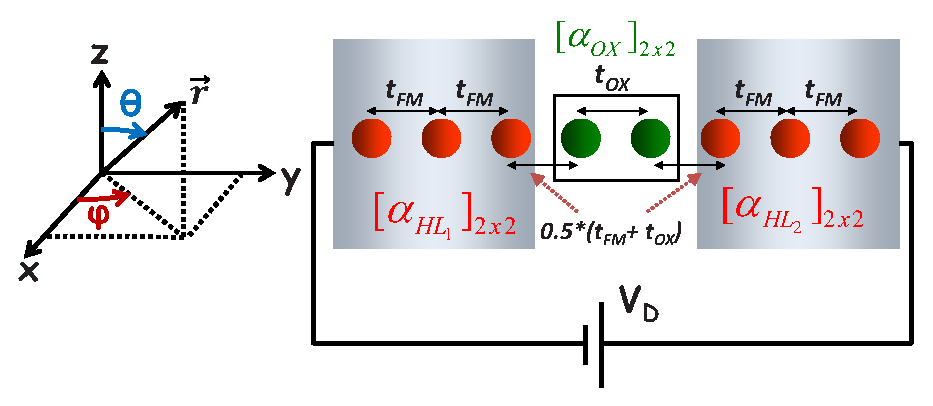
\includegraphics[scale=0.75]{ResearchNotes_NEGF/figs/simframe/negf_grid.eps}
\caption{Illustration of the reference axis (left) and Non-Equilibrium Green's Function based description of the magnetic tunnel junction (right). The reference axis shows how magnetization angles are named in this work. The coupling between lattice sites are $t_{FM}$ and $t_{OX}$ and individual lattice sites are described by the Hamiltonian $\alpha_{HL1}$, $\alpha_{HL2}$ and $\alpha_{OX}$. The complete Hamiltonian describing the MTJ is written in terms of $t_{FM}$, $t_{OX}$, $\alpha_{HL1}$, $\alpha_{HL2}$ and $\alpha_{OX}$.}
\label{fig:negf_grid}
\end{figure}\begin{figure}[!t]
\centering
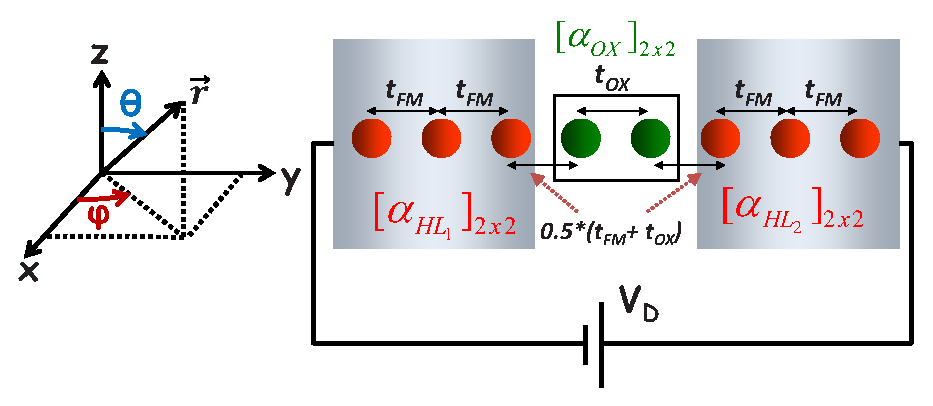
\includegraphics[scale=0.75]{ResearchNotes_NEGF/figs/simframe/negf_grid.eps}
\caption{Temp holder}
\label{fig:bandDiags}
\end{figure}
\clearpage
}\begin{IEEEeqnarray}{rCl}
\alpha_{HL1}&=&\alpha_{FM,L} = 2t_{FM,Left}I \\
\alpha_{HL2}&=&\alpha_{FM,R} = 2t_{FM,Right}I \\
\alpha_{OX}&=&\alpha_{Ch} = 2t_{OX}I \\
\alpha_{IL}&=&\frac{\alpha_{OX}+\alpha_{FM,L}}{2} \\
\alpha_{IR}&=&\frac{\alpha_{OX}+\alpha_{FM,R}}{2} \\
\beta_{HL1}&=&\beta_{FM,L} = -t_{FM,Left}I \\
\beta_{HL2}&=&\beta_{FM,R} = -t_{FM,Right}I \\
\beta_{OX}&=&-t_{OX}I
\end{IEEEeqnarray} where $I$ is the $2\times{}2$ identity matrix. Then, effective masses are used to write \begin{IEEEeqnarray}{rCl}
t_{FM,Left}&=&\frac{\hbar^{2}}{2m^{*}_{FM,Left}a^{2}} \\
t_{FM,Right}&=&\frac{\hbar^{2}}{2m^{*}_{FM,Right}a^{2}} \\
t_{OX}&=&\frac{\hbar^{2}}{2m^{*}_{OX}a^{2}}
\end{IEEEeqnarray}where $a$ is the uniform grid spacing, $\hbar=\frac{h}{2\pi}$ is the reduced Planck constant, and $m^{*}_{OX}$, $m^{*}_{FM,Left}$, and $m^{*}_{FM,Right}$ are the effective electron masses in the oxide channel, the left FM contact, and the right FM contact, respectively. Note that the on-site energy at every grid point is represented by a $2\times{}2$ matrix to handle the spin degeneracy when $\mathcal{H}$ is written this way.

In a ferromagnetic material, the conduction bands for up-spin and down -spin electrons are split. As illustrated in Fig.~\ref{fig:bandDiags}, $U_{b}$ is the barrier height of the tunnel barrier, and $\Delta_{L}$ and $\Delta_{R}$ are the splitting energies between the bottom of the conduction bands for up-spin and down-spin electrons in the left FM contact and right FM contact, respectively. The potential barrier of the tunnel oxide is included in $\mathcal{H}$ by writing \begin{IEEEeqnarray}{rCl}
\alpha_{OX}&=&\alpha_{Ch}+U_{b}I \\
\alpha_{IL}&=&0.5\times\left(\alpha_{OX}+\alpha_{FM,L}+U_{b}\right) \\
\alpha_{IR}&=&0.5\times\left(\alpha_{OX}+\alpha_{FM,R}+U_{b}\right)
\end{IEEEeqnarray}where $I$ is the $2\times{}2$ identity matrix. Then, to include the conduction band splitting, we rewrite \begin{IEEEeqnarray}{rCl}
\alpha_{HL1}&=&\alpha_{FM,L}+U_{split,L} \\
\alpha_{HL2}&=&\alpha_{FM,R}+U_{split,R} \\
\alpha_{IL}&=&0.5\times\left(\alpha_{OX}+\alpha_{FM,L}+U_{b}+U_{split,L}\right) \\
\alpha_{IR}&=&0.5\times\left(\alpha_{OX}+\alpha_{FM,R}+U_{b}+U_{split,R}\right) \\
U_{split,L}&=&\begin{bmatrix}
0 & 0 \\
0 & \Delta_{L}
\end{bmatrix} \label{eq:onsiteL} \\
U_{split,R}&=&\begin{bmatrix}
0 & 0 \\
0 & \Delta_{R}
\end{bmatrix} \label{eq:onsiteR}
\end{IEEEeqnarray}Eqs.~(\ref{eq:onsiteL}) and (\ref{eq:onsiteR}) are written assuming the magnetization directions of the left and right FM contacts are the same and are pointing in the $+\widehat{z}$ direction of the reference frame. If they are different, we may choose one of the FM contacts (e.g., left FM contact) to be the reference frame and define its magnetization direction to be the $+\widehat{z}$ direction. Using the left FM contact as the reference frame, the magnetization direction of the right FM contact, $\widehat{m}$, may be written. In this example, a unitary transformation needs to be performed on $U_{split,R}$ to rewrite it as \begin{equation}
U_{split,R} = \frac{\left(I-\vv{\sigma}\cdot\widehat{m}\right)\Delta_{R}}{2} \label{eq:unitaryTrans}
\end{equation}where $\vv{\sigma}$ is the vector of Pauli spin matrices. Note that for any arbitrarily chosen reference frame, unitary transformation is performed on both $U_{split,L}$ and $U_{split,R}$, using $\widehat{m}$ to be the magnetization vector direction for the corresponding ferromagnetic contact in the chosen reference frame. By definition, the dot product in Eq.~(\ref{eq:unitaryTrans}) yields a $2\times{}2$ matrix that is a linear combination of the Pauli spin matrices given by \begin{equation}
\vv{\sigma}\cdot\widehat{m} = m_{x}\vv{\sigma}_{x}+m_{y}\vv{\sigma}_{y}+m_{z}\vv{\sigma}_{z}
\end{equation}where the components of the vectors have been explicitly written. Note that unitary transformations acting on identity matrices does not do anything. Hence, only $U_{split,L}$ and $U_{split,R}$ needs to be modified to obtain $\mathcal{H}$ when any of the magnetizations do not point along the $+\widehat{z}$ direction of the chosen reference frame.

The applied voltage across the MTJ modifies the potential profile along the longitudinal direction of the MTJ and may be modeled as $U_{V}$. The non-zero entries of $U_{V}$ are on its main diagonal and may be calculated using \begin{equation}
U_{V}(i,i)=\left\lbrace \,
\begin{IEEEeqnarraybox}[][c]{l?s}
\frac{qV}{2}I & if $i$ is in $HL1$ or $IL$, \\
\frac{-qV}{2}I & if $i$ is in $HL2$ or $IR$, \\
qV\left(\frac{1}{2}-\frac{i}{N+1}\right)I & if $i$ is in $OX$.
\end{IEEEeqnarraybox} \right.
\end{equation}where $N$ is the total number of grid points in the OX region. Next, the full Hamiltonian, $\mathcal{H}_{Full}$, is written as \begin{equation}
\mathcal{H}_{Full}=\mathcal{H}+U_{V}
\end{equation}

The self-energy matrices, $\Sigma_{L,R}$, represent the coupling of the external system to the contacts. Based on the construction of $\mathcal{H}_{Full}$,  the non-zero components $\Sigma_{L}$ and $\Sigma_{R}$ are on the top left and bottom right, respectively. The non-zero parts of the self-energies may be written as \begin{equation}\label{eq:self_energyL}
\Sigma_{L}=
\begin{bmatrix}
-t_{FM,Left}exp\left(-ik_{L}^{\uparrow}a\right) & 0 \\
0 & -t_{FM,Left}exp\left(-ik_{L}^{\downarrow}a\right)
\end{bmatrix}
\end{equation}\begin{equation}\label{eq:self_energyR}
\Sigma_{R}=
\begin{bmatrix}
-t_{FM,Right}exp\left(-ik_{R}^{\uparrow}a\right) & 0 \\
0 & -t_{FM,Right}exp\left(-ik_{R}^{\downarrow}a\right)
\end{bmatrix}
\end{equation} where \begin{equation}
k_{L}^{\uparrow}=cos^{-1}\left(1-\frac{E+\frac{qV}{2}}{2t_{FM,Left}} \right)
\end{equation}\begin{equation}
k_{R}^{\uparrow}=cos^{-1}\left(1-\frac{E-\frac{qV}{2}}{2t_{FM,Right}} \right)
\end{equation}\begin{equation}
k_{L}^{\downarrow}=cos^{-1}\left(1-\frac{E+\frac{qV}{2}-\Delta_{L}}{2t_{FM,Left}} \right)
\end{equation}\begin{equation}
k_{R}^{\downarrow}=cos^{-1}\left(1-\frac{E-\frac{qV}{2}-\Delta_{R}}{2t_{FM,Right}} \right)
\end{equation}$E$ is the energy level of interest. This form of Eqs.~(\ref{eq:self_energyL}) and (\ref{eq:self_energyR}) are used if the magnetization direction is in the $+\widehat{z}$ direciton. As before, a unitary transformation needs to be performed on $\Sigma_{L,R}$ of the FM contact whose magnetization direction is not in the $+\widehat{z}$ direciton of the reference frame. The matrix for unitary transformation is given by \begin{equation}
\Lambda_{trans} =
\begin{bmatrix}
cos\left(\frac{\theta}{2}\right)exp\left(i\frac{\phi}{2}\right) & sin\left(\frac{\theta}{2}\right)exp\left(-i\frac{\phi}{2}\right) \\
-sin\left(\frac{\theta}{2}\right)exp\left(i\frac{\phi}{2}\right) & cos\left(\frac{\theta}{2}\right)exp\left(-i\frac{\phi}{2}\right) \\
\end{bmatrix}
\end{equation} where $\theta$ and $\phi$ correspond to the spherical angles of the magnetization vector direction to the Cartesian axis in the reference frame. The self-energy matrices are transformed using \begin{equation}
\Sigma_{L,R}^{new}=\Lambda_{trans}\Sigma_{L,R}^{old}\Lambda_{trans}^{\dagger}
\end{equation}

With the Hamiltonian ($\mathcal{H}_{Full}$) and the self-energy matrices ($\Sigma_{L,R}$), all quantities of interest may be calculated from the following:
\begin{align}
\textbf{Green's function: } G(E) &= (EI - \mathcal{H}_{Full} - \Sigma_L - \Sigma_R)^{-1} \\
\textbf{Spectral density: } A &= i(G-G^{\dagger})=G \Gamma G^{\dagger} \\
\textbf{Electron correlation function: } G^{n}(E) &= G(\Sigma_{L}^{in} + \Sigma_{R}^{in})G^{\dagger} \label{eq:eCorrFunc} \\
\textbf{In-scattering function: } \Sigma_{L,R}^{in}(E) &= \Gamma_{L,R}(E)f_{L,R}(E) \\
\textbf{Broadening matrix: } \Gamma_{L,R}(E) &= i(\Sigma_{L,R} - \Sigma_{L,R}^{\dagger})
\end{align} The diagonal elements of $A$ and $G^n$ correspond to the local density of states and electron density, respectively. $\Sigma^{in}$ is the in-scattering function describing the rate at which electrons enter the device from the $L$ and $R$ contacts, and $f_{L,R}(E)$ are the Fermi functions in the $L$ and $R$ contacts. \begin{IEEEeqnarray}{rCl}
f_{L}(E)&=&\frac{1}{1+exp\left(\frac{E-\mu_{L}}{k_{B}T}\right)} \\
f_{R}(E)&=&\frac{1}{1+exp\left(\frac{E-\mu_{R}}{k_{B}T}\right)}
\end{IEEEeqnarray}where $k_{B}$ is the Boltzmann constant, $T$ is the absolute temperature of the system, and $\mu_{L}$ and $\mu_{R}$ are the electrochemical potential of the left and right FM contacts, respectively. The charge and spin currents flowing through the MTJ are then calculated using
\begin{center}
\textbf{\underline{Charge current density}}
\end{center}
\begin{equation}\label{eq:negf_jcurr}
J_{k,k+1} = Real \left(\frac{1}{i\hbar} \int_{E} \left( Trace \left(\mathcal{H}_{Full,k,k+1}G_{k+1,k}^n - G_{k,k+1}^n\mathcal{H}_{Full,k+1,k} \right)\right) dE \right)
\end{equation}\begin{center}
\textbf{\underline{Spin current density}}
\end{center}
\begin{equation}\label{eq:negf_js}\begin{aligned}
\vv{J}_{S} &= J_{k,k+1}^{Spin} \\
&= Real \left(\frac{1}{i2e\mu_{0}M_{S}V_{magnet}} \int_{E} \left( Trace \left\lbrace \widehat{\sigma} \cdot \left(\mathcal{H}_{Full,k,k+1}G_{k+1,k}^n - G_{k,k+1}^n\mathcal{H}_{Full,k+1,k} \right)\right\rbrace\right) dE \right)
\end{aligned}\end{equation} where $G^n$ is the electron correlation function calculated as given by Eq.~(\ref{eq:eCorrFunc}), $e$ is the elementary charge, $\mu_{0}$ is the permeability of vacuum, $M_{S}$ and $V_{magnet}$ is the saturation magnetization and volume of the magnetic layer the torque is acting on in the MTJ. The charge and spin currents calculated using the NEGF approach are used to determine the spin-transfer torque exerted on the free ferromagnetic layer of the MTJ.

\section{Extending the 1-D model to higher dimension systems}\label{sec:extendDim}

The model presented thus far only models the electron transport in the MTJ considered as a 1-D wire. In real devices, the lateral dimensions may be substantially larger and hence, the 1-D model may not apply. However, the methodology above can still be used for systems with higher order dimensions. The Hamiltonian is written differently for 2-D and for 3-D systems. Let us consider the a 2-D MTJ first. The same approach presented earlier may be used to write $\mathcal{H}$, except that $\alpha_{HL1}$, $\alpha_{HL2}$, $\alpha_{IL}$, $\alpha_{IR}$ , $\alpha_{OX}$, $\beta_{HL1}$, $\beta_{HL2}$, $\beta_{IL}$, $\beta_{IR}$, and $\beta_{OX}$ needs to be rewritten. Assume that $N_{t}$ grid points lie in the \emph{transverse} direction (the direction perpendicular to the longitudinal direction). First, note that every line of grid points in the transverse direction lie in only one of the five defined regions. Using the left FM contact as an example, we rewrite \begin{IEEEeqnarray}{rCl}
\alpha_{HL1}&=&\left[ \begin{IEEEeqnarraybox}[][c]{/c/c/c/c/c/}
2\alpha_{FM,L} & \beta_{FM,L} & 0 & \cdots & 0 \\
\beta^{\dagger}_{FM,L} & \ddots & \ddots & \ddots & \vdots \\
0 & \ddots & \ddots & \ddots & 0 \\
\vdots &\ddots & \ddots & \ddots & \beta_{FM,L} \\
0 & \cdots & 0 & \beta^{\dagger}_{FM,L} & 2\alpha_{FM,L}
\end{IEEEeqnarraybox}\right] \label{eq:modAlph2d} \\
\beta_{HL1}&=&-t_{FM,Left}I \label{eq:modBeta2d}
\end{IEEEeqnarray}where $I$ is the $2N_{t}\times2N_{t}$ identity matrix. To account for the conduction splitting, $U_{split,L}$ is added to every $2\times{}2$ entry on the main diagonal of $\alpha_{HL1}$. The same approach is used to modify $\alpha_{HL2}$ and $\beta_{HL2}$. $\alpha_{OX}$ and $\beta_{OX}$ are modified using the same approach given in Eqs.~(\ref{eq:modAlph2d}) and (\ref{eq:modBeta2d}), except that $U_{b}I$ is added to every $2\times{}2$ entry on the main diagonal of $\alpha_{OX}$. Then, \begin{IEEEeqnarray}{rCl}
\alpha_{IL}&=&0.5\times\left(\alpha_{HL1}+\alpha_{OX}\right) \\
\alpha_{IR}&=&0.5\times\left(\alpha_{HL2}+\alpha_{OX}\right)
\end{IEEEeqnarray}The rewritten $\alpha_{HL1}$, $\alpha_{HL2}$, $\alpha_{IL}$, $\alpha_{IR}$ , $\alpha_{OX}$, $\beta_{HL1}$, $\beta_{HL2}$, and $\beta_{OX}$ are then used to write $\mathcal{H}$ as given by Eq.~(\ref{eq:genHam}).

In a 3-D system, transverse directions forms a 2-D plane of grid points. Hence, $\alpha_{HL1}$, $\alpha_{HL2}$, $\alpha_{IL}$, $\alpha_{IR}$ , $\alpha_{OX}$, $\beta_{HL1}$, $\beta_{HL2}$, $\beta_{IL}$, $\beta_{IR}$, and $\beta_{OX}$ each models a 2-D plane of grid points. Consider a 2-D plane in the $HL1$ region with $N_{t1}\times{}N_{t2}$ number of grid points. We write along the direction with $N_{t1}$ points\begin{IEEEeqnarray}{rCl}
\alpha_{1D,HL1}&=&\left[ \begin{IEEEeqnarraybox}[][c]{/c/c/c/c/c/}
3\alpha_{FM,L} & \beta_{FM,L} & 0 & \cdots & 0 \\
\beta^{\dagger}_{FM,L} & \ddots & \ddots & \ddots & \vdots \\
0 & \ddots & \ddots & \ddots & 0 \\
\vdots &\ddots & \ddots & \ddots & \beta_{FM,L} \\
0 & \cdots & 0 & \beta^{\dagger}_{FM,L} & 3\alpha_{FM,L}
\end{IEEEeqnarraybox}\right] \label{eq:modAlph2d_alt} \\
\beta_{1D,HL1}&=&-t_{FM,Left}I \label{eq:modBeta2d_alt}
\end{IEEEeqnarray}where $I$ in Eq.~(\ref{eq:modBeta2d_alt}) is the $2N_{t1}\times2N_{t1}$ identity matrix and $\alpha_{1D,HL1}$ is a $2N_{t1}\times2N_{t1}$ matrix. We can then write \begin{IEEEeqnarray}{rCl}
\alpha_{HL1}&=&\left[ \begin{IEEEeqnarraybox}[][c]{/c/c/c/c/c/}
\alpha_{1D,HL1} & \beta_{1D,HL1} & 0 & \cdots & 0 \\
\beta^{\dagger}_{1D,HL1} & \ddots & \ddots & \ddots & \vdots \\
0 & \ddots & \ddots & \ddots & 0 \\
\vdots &\ddots & \ddots & \ddots & \beta_{1D,HL1} \\
0 & \cdots & 0 & \beta^{\dagger}_{1D,HL1} & \alpha_{1D,HL1}
\end{IEEEeqnarraybox}\right] \label{eq:modAlph3d} \\
\beta_{HL1}&=&-t_{FM,Left}I\label{eq:modBeta3d}
\end{IEEEeqnarray}where $I$ in Eq.~(\ref{eq:modBeta3d}) is the $(2N_{t1}N_{t2})\times(2N_{t1}N_{t2})$ identity matrix and $\alpha_{HL1}$ is a $(2N_{t1}N_{t2})\times(2N_{t1}N_{t2})$ matrix. To account for the conduction band splitting between up-spin and down-spin electrons, $U_{split,L}$ is added to every $2\times2$ entry along the main diagonal of $\alpha_{HL1}$. The same approach is used to rewrite $\alpha_{HL2}$ and $\beta_{HL2}$. $\alpha_{OX}$ is rewritten as prescribed by Eqs.~(\ref{eq:modAlph2d_alt}) and (\ref{eq:modAlph3d}), while $\beta_{OX}$ is rewritten as prescribed by Eqs.~(\ref{eq:modBeta2d_alt}) and (\ref{eq:modBeta3d}). However, $U_{b}I$, where $I$ here is the $2\times2$ identity matrix, is added to every $2\times2$ entry along the main diagonal of $\alpha_{OX}$. Also, just like in the 2-D system, the interfaces are modeled as \begin{IEEEeqnarray}{rCl}
\alpha_{IL}&=&0.5\times\left(\alpha_{HL1}+\alpha_{OX}\right) \\
\alpha_{IR}&=&0.5\times\left(\alpha_{HL2}+\alpha_{OX}\right)
\end{IEEEeqnarray}The rewritten $\alpha_{HL1}$, $\alpha_{HL2}$, $\alpha_{IL}$, $\alpha_{IR}$ , $\alpha_{OX}$, $\beta_{HL1}$, $\beta_{HL2}$, and $\beta_{OX}$ are then used to write $\mathcal{H}$ as given by Eq.~(\ref{eq:genHam}).

\section{The mode space approach}

Note the size of $\mathcal{H}$ grows quadratically with the total number of grid points. As the number of dimensions of the system increases, the size of $\mathcal{H}$ quickly increases as well. Clearly, there may not be enough computer memory to accommodate the numerical program for solving large 3-D systems. Fortunately, the problem for 2-D and 3-D systems may be reduced to multiple 1-D problems using the mode space approach, which drastically reduces the memory requirement for the numerical program. The main reason that allows us to reduce the number of dimensions is that the solutions to the Schr\"odinger equation for the MTJ system may be written as \begin{equation}
\psi_{i}=\psi_{0}\cdot{}exp(i\vv{r}\cdot\vv{k}_{\perp})\cdot{}exp(i\vv{r}\cdot\vv{k}_{\parallel})
\end{equation}where $i=\sqrt{-1}$, $\vv{k}_{\perp}$ is the longitudinal wave vector, and $\vv{k}_{\parallel}$ is the transverse wave vector. In other words, $\alpha_{HL1}$, $\alpha_{HL2}$, $\alpha_{OX}$, $\alpha_{IL}$ and $\alpha_{IR}$ may be diagonalized and our system of equations going into Eq.~(\ref{eq:genHam}) may be rewritten such that \begin{IEEEeqnarray}{rCl}
\alpha_{HL1}&=&2t_{FM,Left}I + E_{t} \\
\alpha_{HL2}&=&2t_{FM,Right}I + \frac{E_{t}t_{FM,Left}}{t_{FM,Right}} \\
\alpha_{OX}&=&2t_{OX}I + \frac{E_{t}t_{FM,Left}}{t_{OX}} \\
\alpha_{IL}&=&(t_{FM,Left}+t_{OX})I + \frac{2E_{t}t_{FM,Left}}{(t_{FM,Left}+t_{OX})} \\
\alpha_{IR}&=&(t_{FM,Right}+t_{OX})I + \frac{2E_{t}t_{FM,Left}}{(t_{FM,Right}+t_{OX})} \\
\beta_{HL1}&=&-t_{FM,Left}I \\
\beta_{HL2}&=&-t_{FM,Right}I \\
\beta_{OX}&=&-t_{OX}I \\
E_{t}(j,j)&=&\frac{\hbar^{2}\left|\vv{k}_{\parallel}(j,j)\right|^{2}}{2m^{*}_{FM,L}}
\end{IEEEeqnarray}The non-zero entries of $E_{t}$ are on its main diagonal, and $I$ is the identity matrix. The size of $I$ is such that the number of entries along each row and column corresponds to twice the number of grid points in the transverse directions of the system. The same system of equations may be solved by considering each $E_{t}$ separately. For each $E_{t}$, $\mathcal{H}$ is written as in the 1-D case but with \begin{IEEEeqnarray}{rCl}
\alpha_{HL1}&=&\alpha_{FM,L} = 2t_{FM,Left}I + E_{t} \\
\alpha_{HL2}&=&\alpha_{FM,R} = 2t_{FM,Right}I + \frac{E_{t}t_{FM,Left}}{t_{FM,Right}}\\
\alpha_{OX}&=&\alpha_{Ch} = 2t_{OX}I + \frac{E_{t}t_{FM,Left}}{t_{OX}} \\
\alpha_{IL}&=&\frac{\alpha_{OX}+\alpha_{FM,L}}{2} \\
\alpha_{IR}&=&\frac{\alpha_{OX}+\alpha_{FM,R}}{2} \\
\beta_{HL1}&=&\beta_{FM,L} = -t_{FM,Left}I \\
\beta_{HL2}&=&\beta_{FM,R} = -t_{FM,Right}I \\
\beta_{OX}&=&-t_{OX}I
\end{IEEEeqnarray} where $I$ is the $2\times{}2$ identity matrix.

The transverse mode energies, $E_{t}$, depends on the dimensionality of the system, the number of transverse grid points, and the type of boundary conditions. In Section~\ref{sec:extendDim}, we have written $\mathcal{H}$ using box boundary conditions. Let us consider the 2-D case first. It turns out that we may write the mode energies as \begin{IEEEeqnarray}{rCl}
E_{t}&=&2t_{FM,Left}\times\left(1-cos\left(k_{\parallel}a\right)\right)
\end{IEEEeqnarray}When the box boundary condition is used, the plane wave solution to the Schr\"odinger equation must be periodic in the transverse direction. Furthermore, it must go to zero at both ends along the transverse direction due to box boundary conditions. Hence, we can write the plane wave solution as \begin{IEEEeqnarray}{rCl}
\Psi_{\nu}&=&\Psi_{0}exp\left(ik_{\perp}l_{\perp}\right)sin(k_{\parallel}l_{\parallel}) \\
k_{\parallel}(N_{t}+1)a &=& \nu\pi \text{~when~}l_{\parallel}=(N_{t}+1)a
\end{IEEEeqnarray}where $\nu$ is an integer in [1, $N_{t}$] and $N_{t}$ is the number of grid points in the transverse direction. Then,\begin{IEEEeqnarray}{rCl}
E_{t}&=&2t_{FM,Left}\times\left(1-cos\left(\frac{\nu\pi}{N_{t}+1}\right)\right)
\end{IEEEeqnarray} On the other hand, periodic boundary conditions (\emph{pbc}) may also be used to model devices where the characteristic does not depend on the boundary condition. When using \emph{pbc}, $\alpha_{HL1}$ is written as \begin{IEEEeqnarray}{rCl}
\alpha_{HL1}&=&\left[\begin{IEEEeqnarraybox}[][c]{/c/c/c/c/c/c/}
2\alpha_{FM,L} & \beta_{FM,L} & 0 & \cdots & 0 & \beta^{\dagger}_{FM,L} \\ 
\beta^{\dagger}_{FM,L} & \ddots & \ddots & \ddots & \ddots & 0 \\ 
0 & \ddots & \ddots & \ddots & \ddots & \vdots \\ 
\vdots & \ddots & \ddots & \ddots & \ddots & 0 \\ 
0 & \ddots & \ddots & \ddots & \ddots & \beta_{FM,L} \\ 
\beta_{FM,L} & 0 & \cdots & 0 & \beta^{\dagger}_{FM,L} & 2\alpha_{FM,L} 
\end{IEEEeqnarraybox}\right]
\end{IEEEeqnarray}and similarly for $\alpha_{HL2}$, $\alpha_{IL}$, $\alpha_{IR}$ , and $\alpha_{OX}$. The plane wave solution to the Schr\"odinger equation is only required to be periodic in the transverse direction. Hence, \begin{IEEEeqnarray}{rCl}
\Psi_{\nu}&=&\Psi_{0}exp\left(ik_{\perp}l_{\perp}\right)exp(ik_{\parallel}l_{\parallel}) \\
k_{\parallel}(N_{t})a &=& 2\nu\pi \text{~when~} l_{\parallel}=N_{t}a
\end{IEEEeqnarray}where $\nu$ is an integer in [1, $N_{t}$] and $N_{t}$ is the number of grid points in the transverse direction. Then,\begin{IEEEeqnarray}{rCl}
E_{t}&=&2t_{FM,Left}\times\left(1-cos\left(\frac{2\nu\pi}{N_{t}}\right)\right)
\end{IEEEeqnarray}

The transverse mode energies for 3-D systems may be constructed from the same approach we just described. Let us consider the longitudinal direction to be in the $+\widehat{z}$ direction, and the transverse directions to be $+\widehat{x}$ and $+\widehat{y}$. Furthermore, assume there are $N_{t1}$ and $N_{t2}$ grid points in the $x$ and $y$ directions, respectively. We invoke the fact that plane wave solutions to the Schr\"odinger equation have the form \begin{equation}
\Psi_{\nu} = \Psi_{0}e^{i\left(k_{x}r_{x} + k_{y}r_{y} + k_{z}r_{z}\right)}
\end{equation}Since $k_{x}$ and $k_{y}$ are decoupled, the combined transverse mode energy is a linear combination of every permutation of the transverse mode energy in the $x$ and $y$ direction ($E_{t,x}$ and $E_{t,y}$, respectively). Hence, every $E_{t,x}$ and $E_{t,y}$ are first obtained by choosing integers $\nu_{x}$ and $\nu_{y}$ in the range [1, $N_{t1}$] and [1, $N_{t2}$], respectively. If both directions have box boundary conditions, then we can write \begin{IEEEeqnarray}{rCl}
E_{t,x}&=&2t_{FM,Left}\times\left(1-cos\left(\frac{\nu_{1}\pi}{N_{t1}+1}\right)\right) \\
E_{t,y}&=&2t_{FM,Left}\times\left(1-cos\left(\frac{\nu_{2}\pi}{N_{t2}+1}\right)\right)
\end{IEEEeqnarray}and calculate $E_{t}=E_{t,x}+E_{t,y}$ using every permutation of $E_{t,x}$ and $E_{t,y}$. If both directions have \emph{pbc}, then use \begin{IEEEeqnarray}{rCl}
E_{t,x}&=&2t_{FM,Left}\times\left(1-cos\left(\frac{2\nu_{1}\pi}{N_{t1}}\right)\right) \\
E_{t,y}&=&2t_{FM,Left}\times\left(1-cos\left(\frac{2\nu_{2}\pi}{N_{t2}}\right)\right)
\end{IEEEeqnarray}instead. If the box boundary condition is applied along the $x$ direction but \emph{pbc} along the $y$ direction, then use \begin{IEEEeqnarray}{rCl}
E_{t,x}&=&2t_{FM,Left}\times\left(1-cos\left(\frac{\nu_{1}\pi}{N_{t1}+1}\right)\right) \\
E_{t,y}&=&2t_{FM,Left}\times\left(1-cos\left(\frac{2\nu_{2}\pi}{N_{t2}}\right)\right)
\end{IEEEeqnarray}instead. If the box boundary condition is applied along the $y$ direction but \emph{pbc} along the $x$ direction, then use \begin{IEEEeqnarray}{rCl}
E_{t,x}&=&2t_{FM,Left}\times\left(1-cos\left(\frac{2\nu_{1}\pi}{N_{t1}}\right)\right) \\
E_{t,y}&=&2t_{FM,Left}\times\left(1-cos\left(\frac{\nu_{2}\pi}{N_{t2}+1}\right)\right)
\end{IEEEeqnarray} The charge and spin currents flowing through the MTJ are calculated for each mode and all contributions are summed together to obtain the actual charge and spin current flowing through the MTJ, giving 
\begin{center}
\textbf{\underline{Charge current density}}
\end{center}
\begin{equation}\label{eq:negf_jcurr_modeDis}
J_{k,k+1} = \sum_{E_{t}} Real \left(\frac{1}{i\hbar} \int_{E_{z}} \left( Trace \left(\Upsilon \right)\right) \partial{}E_{z} \right)
\end{equation}\begin{center}
\textbf{\underline{Spin current density}}
\end{center}
\begin{equation}\label{eq:negf_js_modeDis}
\vv{J}_{S} = \sum_{E_{t}} Real \left(\frac{1}{i2e\mu_{0}M_{S}V_{magnet}} \int_{E_{z}} \left( Trace \left\lbrace \widehat{\sigma} \cdot \Upsilon\right\rbrace\right) \partial{}E_{z} \right)
\end{equation}where $\Upsilon$ is given by\begin{equation}
\Upsilon=\mathcal{H}_{Full,k,k+1}(E_{t})G_{k+1,k}^n(E_{t}) - G_{k,k+1}^n(E_{t})\mathcal{H}_{Full,k+1,k}(E_{t})
\end{equation}and $\mathcal{H}_{Full}$ and $G^{n}$ are now functions of $E_{t}$.

\section{Approximating mode space calculations in NEGF}\label{sec:negf_Soln}

In MTJs, the Fermi level in the FM contacts are deep inside the conduction band and as a result, the grid spacing may need to be very small in order for the numerical solutions to converge (even in the 1-D case). Even for MTJs with $10~\text{nm}\times10~\text{nm}$ cross-sectional area, the number of transverse modes needed to be considered to calculate its $I-V$ characteristic can be in the tens of thousands. Since the NEGF calculations for each transverse mode energy is independent of the others, the numerical simulation can be easily parallelized and executed on a large computer cluster to obtain the results quickly. However, because the data needs to be communicated to every computing node in the cluster, the simulation might be slowed down if the network traffic is too heavy. To overcome this issue, we first note that when the MTJ size is sufficiently large, the number of transverse modes in $k$-space is very dense. Hence, it may be possible to turn the discrete summation in Eqs.~(\ref{eq:negf_jcurr_modeDis}) and (\ref{eq:negf_js_modeDis}) into a continuous integral. This approach was proposed in \cite{Duke1969} and was used by Tsu-Esaki to model resonant tunneling diodes \cite{Tsu1973a}.

When we change the summation over modes in 3-D to a continuous integration, it can be converted as \begin{equation}
\sum_{E_{t,x}}\sum_{E_{t,y}}\sum_{E_{t,z}} \rightarrow \int\int\int\partial{}k_{x}\partial{}k_{y}\partial{}k_{z}
\end{equation}However, the triple integral can be converted into a single integral if we integrate over the actual energy of the transverse mode instead. \begin{equation}
\int\int\int\partial{}k_{x}\partial{}k_{y}\partial{}k_{z} \rightarrow \int\partial{}k_{\parallel} \rightarrow DOS(E_{t}) \int\partial{}E_{t}
\end{equation}where $DOS(E_{t})$ is the density of states. This can be done if we know the dispersion relation, which is assumed to be quadratic for most problems \begin{equation}
E_{t} = \frac{\hbar^{2}(\vv{k}\cdot\vv{k})}{2m^{*}_{eff}}=\frac{\hbar^{2}(k^{2}_{x}+k^{2}_{y}+k^{2}_{z})}{2m^{*}_{eff}}=\frac{\hbar^{2}{}k^{2}_{\parallel}}{2m^{*}_{eff}}
\end{equation}where $m^{*}_{eff}$ is the effective mass of the electron. Rearranging, \begin{equation}
k_{\parallel}=\frac{\sqrt{2m^{*}_{eff}E_{t}}}{\hbar} \label{eq:kERel}
\end{equation}We also need to determine $DOS(E_{t})$. In a 3-D box which has \emph{pbc} in all three Cartesian coordinate directions. The $k$-states are separated by \begin{equation}
\Delta{}k_{x}=\frac{\pi}{L_{x}},~\Delta{}k_{y}=\frac{\pi}{L_{y}},~\Delta{}k_{z}=\frac{\pi}{L_{z}}
\end{equation}where $L_{x}$, $L_{y}$ and $L_{z}$ is the length of each side of the confining box. Furthermore, each $k_{x}$, $k_{y}$ and $k_{z}$ falls in the range [$-\pi$, $\pi$]. Hence, in $k$-space, each state occupies a volume given by \begin{equation}
\text{Volume~occupied~by~a~state~in~k-space~for~a~3-D~box}=\frac{2\pi}{L_{x}}\times\frac{2\pi}{L_{y}}\times\frac{2\pi}{L_{z}}=\frac{8\pi^{3}}{\Omega}
\end{equation}where $\Omega=L_{x}L_{y}L_{z}$. To get the \emph{density of states}, we need to determine how many states are uncovered when $E_{t}$ changes to $E_{t}+\partial{}E_{t}$. This corresponds to a change in volume in $k$-space. When $E_{t}$ changes, the volume changes spherically. \begin{table}[!t]
\caption{Summary of $DOS(E_{t})$ calculations}
\centering
\label{tab:DOS}
\begin{IEEEeqnarraybox}[\IEEEeqnarraystrutmode][c]{v/c/v/c/v/c/v/c/v/c/v/c/v}
\IEEEeqnarrayrulerow \\
& \raisebox{-7pt}[0pt][0pt]{Dimensions} && \raisebox{-7pt}[0pt][0pt]{$\Omega$} && \text{Volume~of} && \text{Volume~of~sphere} && \text{Number~of~states} && \raisebox{-7pt}[0pt][0pt]{$DOS(E_{t})$}  \\
& && && \text{one~state} && \text{in~}k\text{-space} && \text{in~sphere} && \\
\IEEEeqnarrayrulerow \\
& \raisebox{-2pt}[0pt][0pt]{3-D} && \raisebox{-2pt}[0pt][0pt]{$L_{x}L_{y}L_{z}$} && \begin{IEEEeqnarraybox}[\IEEEeqnarraystrutsize{24pt}{11pt}][c]{c}\frac{8\pi^{3}}{\Omega}\end{IEEEeqnarraybox} && \begin{IEEEeqnarraybox}[\IEEEeqnarraystrutsize{24pt}{11pt}][c]{c}\frac{4\pi{}k_{\parallel}^{3}}{3}\end{IEEEeqnarraybox} && \begin{IEEEeqnarraybox}[\IEEEeqnarraystrutsize{27pt}{10pt}][c]{c}\frac{\Omega{}\left(2m^{*}_{eff}E_{t}\right)^{\frac{3}{2}}}{6\pi^{2}\hbar^{3}}\end{IEEEeqnarraybox} && \begin{IEEEeqnarraybox}[\IEEEeqnarraystrutsize{20pt}{10pt}][c]{c}\frac{\Omega2\pi(2m^{*}_{eff})^\frac{3}{2}}{h^{3}}\sqrt{E_{t}}\end{IEEEeqnarraybox} \\
\IEEEeqnarrayrulerow \\
& \raisebox{-2pt}[0pt][0pt]{2-D} && \raisebox{-2pt}[0pt][0pt]{$L_{x}L_{y}$} && \begin{IEEEeqnarraybox}[\IEEEeqnarraystrutsize{18pt}{10pt}][c]{c}\frac{4\pi^{2}}{\Omega}\end{IEEEeqnarraybox} && \pi{}k_{\parallel}^{2} && \begin{IEEEeqnarraybox}[\IEEEeqnarraystrutsize{18pt}{10pt}][c]{c}\frac{\Omega2\pi{}m^{*}_{eff}E_{t}}{h^{2}}\end{IEEEeqnarraybox} && \begin{IEEEeqnarraybox}[\IEEEeqnarraystrutsize{18pt}{10pt}][c]{c}\frac{\Omega2\pi{}m^{*}_{eff}}{h^{2}}\end{IEEEeqnarraybox} \\
\IEEEeqnarrayrulerow \\
& \raisebox{-1.5pt}[0pt][0pt]{1-D} && \raisebox{-1.5pt}[0pt][0pt]{$L_{x}$} && \begin{IEEEeqnarraybox}[\IEEEeqnarraystrutsize{18pt}{10pt}][c]{c}\frac{2\pi}{\Omega}\end{IEEEeqnarraybox} && 2k_{\parallel} && \begin{IEEEeqnarraybox}[\IEEEeqnarraystrutsize{21pt}{8.5pt}][c]{c}\frac{\Omega2\sqrt{2m^{*}_{eff}E_{t}}}{h}\end{IEEEeqnarraybox} && \begin{IEEEeqnarraybox}[\IEEEeqnarraystrutsize{21pt}{13pt}][c]{c}\frac{\Omega}{h}\sqrt{\frac{2m^{*}_{eff}}{E_{t}}}\end{IEEEeqnarraybox} \\
\IEEEeqnarrayrulerow
\end{IEEEeqnarraybox}
\end{table}The volume of a sphere is \begin{equation}
Volume = \frac{4\pi{}k_{\parallel}^{3}}{3}
\end{equation}and the total number of states in that volume is \begin{equation}
\text{Number of states~in~volume}=\frac{4\pi{}k_{\parallel}^{3}}{3}\times\frac{\Omega}{8\pi^{3}}=\frac{\Omega{}k_{\parallel}^{3}}{6\pi^{2}} \label{eq:3dspv}
\end{equation}Substituting Eq.~(\ref{eq:kERel}) into (\ref{eq:3dspv}), we get \begin{equation}
\text{Number of states~in~volume}=\frac{\Omega(2m^{*}_{eff}E_{t})^{\frac{3}{2}}}{6\pi^{2}\hbar^{3}}
\end{equation}Then, we can calculate the density of states given as \begin{equation}
DOS(E_{t}) = \frac{\partial}{\partial{}E_{t}} \left(\text{Number of states~in~volume}\right)=\frac{\Omega2\pi(2m^{*}_{eff})^\frac{3}{2}}{h^{3}}\sqrt{E_{t}}
\end{equation}The same process can be repeated to calculate $DOS(E_{t})$ for 2-D and 1-D confinements, and the results are summarized in Table~\ref{tab:DOS}. Note that the number of states in sphere listed in Table~\ref{tab:DOS} is missing a factor of 2 compared to the texts found in the literature. In the literature, the factor of 2 is used to account for degeneracy in energy levels. In the NEGF approach used in this work, the degeneracy is handled by writing $\mathcal{H}$ to include up-spin and down-spin. Hence, the number of states in sphere is as listed in Table~\ref{tab:DOS}. It is important to note the parabolic dispersion relationship assumption used to obtain these results.

Once we obtain $DOS(E_{t})$, we may then calculate the charge and spin currents as \begin{equation}
\Upsilon=\mathcal{H}_{Full,k,k+1}(E_{t})G_{k+1,k}^n(E_{t}) - G_{k,k+1}^n(E_{t})\mathcal{H}_{Full,k+1,k}(E_{t})
\end{equation}
\begin{center}
\textbf{\underline{Charge current density}}
\end{center}
\begin{equation}\label{eq:negf_jcurr_modeCont}
J_{k,k+1} = Real \left(\frac{1}{i\hbar} \int_{E_{t}}\int_{E_{z}} DOS(E_{t})\cdot\left( Trace \left( \Upsilon \right)\right) \partial E_{z} \partial E_{t} \right)
\end{equation}\begin{center}
\textbf{\underline{Spin current density}}
\end{center}
\begin{equation}\label{eq:negf_js_modeCont}
\vv{J}_{S} = Real \left(\frac{1}{i2e\mu_{0}M_{S}V_{magnet}} \int_{E_{t}}\int_{E_{z}} DOS(E_{t})\cdot\left( Trace \left\lbrace \widehat{\sigma} \cdot \Upsilon\right\rbrace\right) \partial E_{z} \partial E_{t} \right)
\end{equation}

Note that we can use the same procedure to determine $DOS(E_{t})$ if box boundary conditions are used. When box boundary conditions are used, the number of $k$-states long each $k$ direction is same as when \emph{pbc} is used. However, the each state is found in [0, $\pi$] instead of [$-\pi$, $\pi$]. It seems as if the volume occupied by each state in $k$-space is smaller. However, the difference in the range over which the states are found needs to be accounted for. In the 3-D case, all $k$-states are in the first octant. In the 2-D case, all $k$-states are in the first quadrant. In the 1-D case, all $k$-states are in the left half. As a result, we get the same number of states in $k$-space sphere regardless of boundary conditions. Hence, $DOS(E_{t})$ is independent of boundary conditions when the grid spacing is sufficiently small. When we simulate an MTJ, we can assume that the electron tunneling probability is independent of the transverse mode energy. Furthermore, we have $L_{x}, L_{y} \geq 10$~nm and the grid spacing needed for numerical results to converge is usually $a\leq0.1$ \AA. Hence, we can approximate the sum over modes as an integral and calculate the charge and spin currents using \begin{center}
\textbf{\underline{Charge current density}}
\end{center}
\begin{equation}\label{eq:negf_jcurr_mode3D}
J_{k,k+1} = Real \left(\frac{m^{*}_{eff}A_{MTJ}}{i2\pi\hbar^{3}} \int_{E_{t}}\int_{E_{z}} \left( Trace \left( \Upsilon \right)\right) \partial E_{z} \partial E_{t} \right)
\end{equation}\begin{center}
\textbf{\underline{Spin current density}}
\end{center}
\begin{equation}\label{eq:negf_js_mode3D}
\vv{J}_{S} = Real \left(\frac{m^{*}_{eff}A_{MTJ}}{i\hbar^{2}4\pi e\mu_{0}M_{S}V_{magnet}} \int_{E_{t}}\int_{E_{z}} \left( Trace \left\lbrace \widehat{\sigma} \cdot \Upsilon\right\rbrace\right) \partial E_{z} \partial E_{t} \right)
\end{equation}where $A_{MTJ}$ is the cross-sectional area of the MTJ.

\section{Using spin current in simulation of magnetization dynamics}

In the free layer of an MTJ, the Landau-Lifshitz-Gilbert (LLG) equation used to model its behavior. The LLG equation is given as \begin{equation}
\frac{\partial\widehat{m}}{\partial t} = -|\gamma| \widehat{m}\times\vv{H}_{eff} + \alpha\left(\widehat{m}\times\frac{\partial\widehat{m}}{\partial t}\right) + \vv{STT}
\end{equation}where $\vv{H}_{eff}$ is the effective magnetic field (including all anisotropy fields, externally applied magnetic fields and magnetostatic field) acting on the free layer, which has a magnetization direction given by $\widehat{m}$. $\gamma$ is the gyromagnetic ratio (usually $2.211\times10^{5}$ m$\cdot$A$^{-1}\cdot$s$^{-1}$) and $\alpha$ is the unitless Gilbert's damping factor. As proposed by Slonczewski \cite{Slonczewski1996c}, the spin-transfer torque is given by \begin{equation}
\vv{STT}=\widehat{m}\times\vv{J}_{S}\times\widehat{m}
\end{equation}where $\vv{J}_{S}$ was given in Eqs.~(\ref{eq:negf_js}), (\ref{eq:negf_js_modeDis}), (\ref{eq:negf_js_modeCont}) and (\ref{eq:negf_js_mode3D}).

